%
% File naacl2019.tex
%
%% Based on the style files for ACL 2018 and NAACL 2018, which were
%% Based on the style files for ACL-2015, with some improvements
%%  taken from the NAACL-2016 style
%% Based on the style files for ACL-2014, which were, in turn,
%% based on ACL-2013, ACL-2012, ACL-2011, ACL-2010, ACL-IJCNLP-2009,
%% EACL-2009, IJCNLP-2008...
%% Based on the style files for EACL 2006 by 
%%e.agirre@ehu.es or Sergi.Balari@uab.es
%% and that of ACL 08 by Joakim Nivre and Noah Smith

\documentclass[11pt,a4paper]{article}
\usepackage[hyperref]{naaclhlt2019}
\usepackage{times}
\usepackage{latexsym}
\usepackage{graphicx}
\graphicspath{ {./images/} }

\usepackage{url}

\aclfinalcopy % Uncomment this line for the final submission
%\def\aclpaperid{***} %  Enter the acl Paper ID here

\setlength\titlebox{9 cm}
% You can expand the titlebox if you need extra space
% to show all the authors. Please do not make the titlebox
% smaller than 5cm (the original size); we will check this
% in the camera-ready version and ask you to change it back.

\newcommand\BibTeX{B{\sc ib}\TeX}

\title{Lyrics Generator: Using Char-Level RNN Model To Generate Lyrics}

\author{Jun Wang \\
  Data Analytics \\
  Georgetown University\\
  Washington, DC, USA \\
 {\tt jw1720@georgetown.edu} 
  \\\
  {\bf Hanlong Peng} \\
  Data Analytics \\
  Georgetown University\\
  Washington, DC, USA \\
  {\tt hp409@georgetown.edu} 
  \\\And
  Pengsen Li \\
  Data Analytics \\
  Georgetown University\\
  Washington, DC, USA \\
  {\tt pl645@georgetown.edu}
  \\\
  {\bf Junke Wang} \\
  Data Analytics \\
  Georgetown University\\
  Washington, DC, USA \\
  {\tt jw1738@georgetown.edu} 
  \\}
  
\date{12/15/2018}

\begin{document}
\maketitle
\begin{abstract}
We present a lyrics generation method with deep learning knowledge to construct a meaningful, interesting lyric story with specific singer's style. The method is based on a character-level RNN with a hidden GRU model as well as a spelling checker function and a timer. We first construct three different numbers of layer for the GRU model (1-layer, 2-layers, and 3-layers) and compare both word-level and char-level accuracy. Results show that 2-layers GRU model provides the highest accuracy percentages - 95.48\% for word-level and 90.97\% for char-level. Second, we try various hidden sizes for the 2-layers GRU model (size of 5, 20, 50, 100, and 200). As a result, a hidden size of 100 and 200 have relatively high accuracy percentages (above 95\% for the word-level and above 91\% for the char-level. Ultimately, the model generates an interesting and mimic short lyric paragraph.

\end{abstract}

\section{Introduction}
Music creation can be tricky since it requires not only the theories from books and experiences from life but also writers creativity and inspiration. Although sophisticated technologies and software are developed for songwriting, it is still hardly possible for any singer or writer to produce great works with a similar style in a frequent and constant rate. The lyrics generator in this research uses the existing lyrics from the songs of a famous singer, Eminem, as its database. We believe that this generator can assist any user to create complete lyrics for a song regardless of talent or creativity. The following sections of this paper will describe in detail about the work in related fields, methods we used, the results from experimenting the methods and a discussion about this research. 

\section{Related Work}
There are various related approaches for lyrics generator problem. Among all the approaches, the most basic and popular methods are Hidden Markov Models and Recurrent Neural Network. One of the best results for generating rap lyrics is from the study conducted by the Hong Kong University of Science and Technology. They published a paper \emph{Unsupervised Rhyme Scheme Identification in Hip Hop Lyrics Using Hidden Markov Models} which is highly related to our project. Karteek Addanki and Dekai Wu introduced a method which is based on a novel hidden Markov model for the completely unsupervised identification of rhyme schemes in hip-hop lyrics. With their highly noise data, they were able to obtain a precision of 57.25\% on identifying the rhyming words with a total F-Score of 44.06\% [1]. Another method created a model based on the RankSVM algorithm and a deep neural network model with a novel structure which is introduced by a group of authors from Finland. Based on their evaluation of the quantitative rhyme density, the method outperforms the best human rappers by 21\%. As a result, their rap lyrics generator has been deployed as an online tool called DeepBeat [2]. Inspired by these two papers with the goal of relating our final project to the deep learning course, we decided to use the Recurrent Neural Network to build our lyrics generator. Then we did more research on this topic. In general, there are two ways of building the model. One is the word-level RNN model and another is char-level RNN model. Therefore, based on our small research we decided to try the char-level RNN and word-level RNN for our project model.


\section{Datasets}
For our dataset, Eminem's songs are selected to be used to train the model. Our final goal is to generate a short Eminem-like rap lyric story. We obtain the Eminem dataset by web scraping. The parser was gathering lyrics from https://www.azlyrics.com/ by requests and beautifulsoup packages in Python. The data was originally stored in a CSV file with song names and lyrics. There are total of 350 songs and some of them are remix versions or music video versions. The data preprocessing process is mainly focused on extracting the lyrics from the raw data and writing them into a new text file.

\section{Method}
\subsection{Evaluation Methods}
Before describing our model, let us first introduce the evaluation methods we pick for this project. Since there is no standard evaluation method the unsupervised learning, we decide to use the spell checker to check the character level and word level accuracy as our own evaluation method. (The word level accuracy is computed by correct number of word divide by the total number of words. Similarly, the character level accuracy is computed by the correct number of character decided by the total number of character.) In addition, we add a timer to see how long does the model take to finish training the dataset. 

\subsection{Word-Level and Char-Level RNN}
We tried both word-level [3] and character-level [4] RNN for our model. For the word level, even though the world level accuracy is 100\% due to the nature of the model, the sentences from the results are monstrous broken and make no sense. On the other hand, for the character-level model, there are some spelling error but the sentences are more coherence and comprehensive. In addition, since there are many low-frequency words in the lyrics dataset, the alphabet dictionary for the word level RNN is really big, and all the low-frequency words would not be able to show in the results. Overall, char-level RNN is able to mimic grammatically correct sequences for a wide range of language, while word-level RNN trains faster and generate more coherent texts which usually do not make actual sense. Also, the main advantage of char-level RNN is that it has a really small vocabulary and it does not require tokenization as a preprocessing step [5]. Ultimately, the final basic model for our lyrics generation task is Char-RNN, which is a recurrent neural network trained to predict the next character given a sequence of precious characters. This could be also explained as a conditional probability distribution to find the most likely character from the alphabet including some other signs. Note that we do not need to tokenize before we define the dictionary of our character alphabet since the model is in character level. When creating training sequences, we set the chunk length of the seed characters equals 200 and each character is typically encoded as a one-hot vector. 

\subsection{Model Parameters}
In practice, the main RNN model we choose is GRU model, which is faster trained than LSTM. We try three different numbers of layers (1-layer, 2-layers, and 3-layers) with the temperature equals 0.7, the hidden size of 100, training epochs of 1000, and batch size of 256. One interesting parameter here is temperature. The temperature is dividing the predicted log probabilities before the Softmax. Thus, a smaller temperature will lead to the model imitating the singer more, but more boring and tedious as well. On the other hands, a larger temperature will make the predicted lyrics more creative and increase the diversity of results, causing more mistakes though. As for our model, the most appropriate temperature is 0.7. 

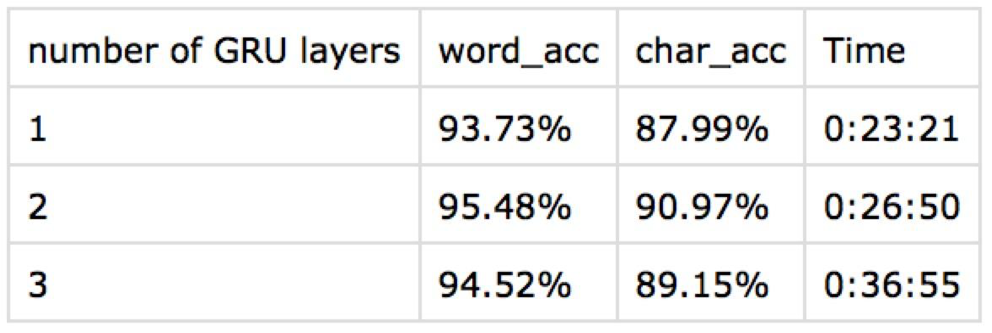
\includegraphics[scale=0.8]{table1.png}
\centerline{Table 1}

Table1 is the word-level and char-level accuracies with time results for the three GRU models. We can see that the 2-layers GRU model provides the best accuracy results both the word accuracy and character accuracy. Also the 3-layers GRU take significant longer time on training. Therefore, we decide to use it as the basic model for the next step. With all parameters fixed in the 2-layers GRU, we change the value for the hidden size for the model. The losses for each epoch are shown in Graph1. The plot is the training loss for different size of the hidden layer. Since these are the losses for the training set, it make sense that the larger hidden size is, the better the model performs. So we take a look at the accuracies and time for each model and Table2 are the resulting outputs.

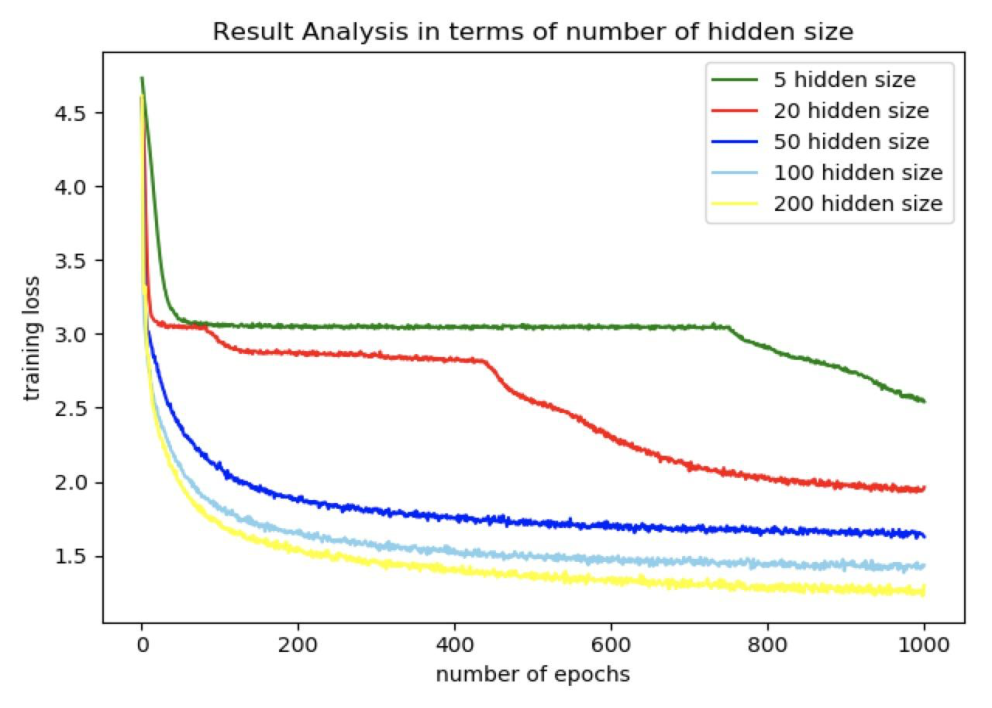
\includegraphics[scale=0.8]{graph1.png}
\centerline{Graph 1}

So we take a look at the accuracies and time for each model and Table2 are the resulting outputs. From the Table2, we can see that hidden size of 100 and 200 both have high accuracies of word-level (above 95\%) and char-level (above 91\%). 

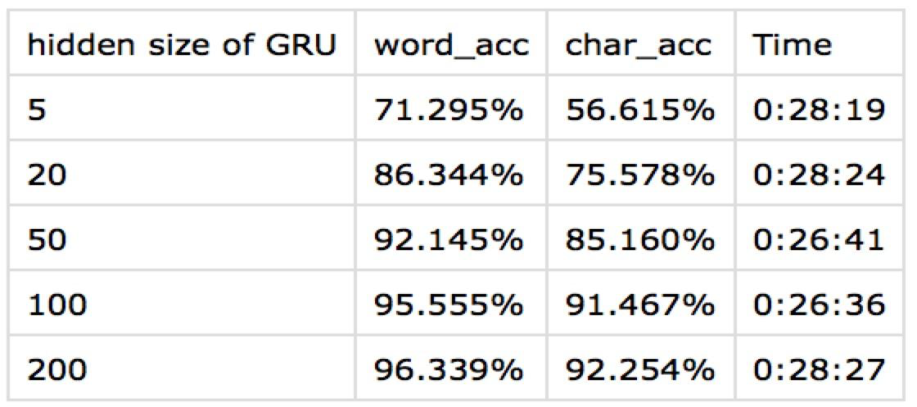
\includegraphics[scale=0.8]{table2.png}
\centerline{Table 2}

Therefore, we choose these two models to generate the Eminem-like Lyrics with the say starting word "Hey" in the Results section.

\section{Results}
\subsection{Lyrics output for hidden size of 100}
\begin{verbatim}
Hey
you money to beful
i shit i don't got a little back, 
i hear the stupid 
so mad you should tell it 
and i do it imma be 
really faking in the honesher 
doubf custom what you know 
you wanna man through the peach
but i can screamings around it, 
so they ha would it gonna see me
and i got down, 
down it past ruthing 
they talk it that?s every gone
what you let?s beginning a hole it, 
I feel hours againma some days 
and vister
and i up and let pocket 
your channipositions 
that with millions
So i can`neal
\end{verbatim}

\subsection{Lyrics output for hidden size of 200}
\begin{verbatim}
Hey
but I just don`t give a fuck 
i wanna take me too, 
she has told you shot
`cause you give`em the new rist 
so we can looks like a fuckin?colla
don`t want you no fame, 
want you no gut
so they say 
they`re just a chuck
and when i go to you, 
but it's just the type of my back
slam with me, 
let on a soldier 
who wanna rock the heck
when i just choke of it, 
it subla cause i smiles 
and shook this head 
while we going to rap
when i`m slim shady
so you just get one control
come on a second shot 
we came off the flow
\end{verbatim}

\section{Discussion of Results}
By comparing the outputs, it is obvious that lyrics from the 200-hidden-layer model is more fluent and natural (with accuracy of 89.05\%). There are misspelling words like 'beful' and 'visiter' in the 100-hidden-layer model and the rhyme is worse (with accuracy of 82.77\%). In order to maintain the lyrics quality, some of the words (rap words) have to be checked manually, like 'Imma', 'skr', 'atchoo' and etc. The final result is a good representation of the evaluation system. It has words like 'imma', 'slim shady', 'subla' that will be treated as wrong spelling but right in rap lyrics. 

\section{Conclusions}
In conclusion, our lyrics generator is the method with the base of character level of RNN with hidden size of 200 and the output lyrics seem really Eminem-like. It is good at maintaining the style of the artist and rap. On the other hand, it is hard to maintain the lyrics quality. For example, a sentence can be incomplete if the input character number is fixed. This is not unexpected because of the natural disadvantage of the char-level RNN due to English is a word based language. In the future, if the rap word detection and the complete sentence detection can be added into the model, the final lyrics output will be much better than now. 



% Min: no longer used as of ACL 2018, following ACL exec's decision to
% remove this extra workflow that was not executed much.
% BEGIN: remove
%% \section{XML conversion and supported \LaTeX\ packages}

%% Following ACL 2014 we will also we will attempt to automatically convert 
%% your \LaTeX\ source files to publish papers in machine-readable 
%% XML with semantic markup in the ACL Anthology, in addition to the 
%% traditional PDF format.  This will allow us to create, over the next 
%% few years, a growing corpus of scientific text for our own future research, 
%% and picks up on recent initiatives on converting ACL papers from earlier 
%% years to XML. 

%% We encourage you to submit a ZIP file of your \LaTeX\ sources along
%% with the camera-ready version of your paper. We will then convert them
%% to XML automatically, using the LaTeXML tool
%% (\url{http://dlmf.nist.gov/LaTeXML}). LaTeXML has \emph{bindings} for
%% a number of \LaTeX\ packages, including the ACL 2018 stylefile. These
%% bindings allow LaTeXML to render the commands from these packages
%% correctly in XML. For best results, we encourage you to use the
%% packages that are officially supported by LaTeXML, listed at
%% \url{http://dlmf.nist.gov/LaTeXML/manual/included.bindings}
% END: remove


\bibliographystyle{stylename}
\bibliography{bibfile}
\medskip
 
\begin{thebibliography}{9}
\bibitem{paper1} 
Karteek Addanki and Dekai Wu.
\textit{Unsupervised Rhyme Scheme Identification in Hip Hop Lyrics Using Hidden Markov Models}.
 Statistical Language and Speech Processing pp. 39-50, 2013.
 
\bibitem{paper2} 
Eric Malmi, Pyry Takala, Hannu Toivonen, Tapani Raiko, and Aristides Gionis. 
\textit{DopeLearning: A Computational Approach to Rap Lyrics Generation}.
Proceedings of the 22nd ACM SIGKDD International Conference on Knowledge Discovery and Data Mining pp. 195-204, 2016.

\bibitem{paper3} 
Enrique A.
\textit{Word-level LSTM text generator. Creating automatic song lyrics with Neural Networks}
https://medium.com/coinmonks/word-level-lstm-text-generator-creating-automatic-song-lyrics-with-neural-networks-b8a1617104fb, 2018

\bibitem{paper4} 
Sean Robertson.
\textit{Training Code for the Char-level RNN Using Pytorch}
https://github.com/spro/char-rnn.pytorch/blob/master/train.py, 2017

\bibitem{paper5} 
StackExchange Question Page.
\textit{What are the main differences between word-based and char-based text generation RNNs}
https://datascience.stackexchange.com/questions/13
138/what-is-the-difference-between-word-based-and-char-based-text-generation-rnns, 2018
\end{thebibliography}


\end{document}
